\section{Introduction}
\label{sec:introduction}

% state the learning objective
\par The objective of this laboratory assignment is to build an Audio Amplifier using a transistor based circuit with a gain stage and an output stage. The circuit can be seen in Figure~\ref{fig:rc}.\\


In Section~\ref{sec:simulation}, the circuit was built ,tested and adjusted to give the expected results.
In Section~\ref{sec:analysis}, it was used the transistor large signal
Ebbers-Moll model  to study the DC component and the transistor small signal
model for the AC component. The results are compared to the simulation results obtained in Section~\ref{sec:simulation}. The conclusions of this study are outlined in
Section~\ref{sec:conclusion}.

\begin{figure}[h] \centering
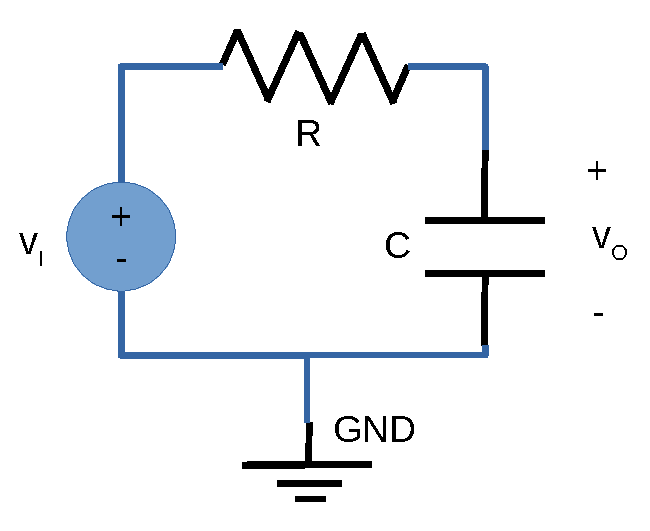
\includegraphics[width=0.65\linewidth]{rc.pdf}
\caption{Audio Amplifier}
\label{fig:rc}
\end{figure}
